\chapter{Bluetooth}

Bluetooth is a wireless technology standard for exchanging data over short distances (using short-wavelength UHF radio waves in the ISM band from 2.4 to 2.485 GHz) from fixed and mobile devices, and building personal area networks (PANs). It was originally conceived as a wireless alternative to RS-232 data cables. Bluetooth is managed by the Bluetooth Special Interest Group (SIG), which has more than 35,000 member companies in the areas of telecommunication, computing, networking, and consumer electronics. The IEEE standardized Bluetooth as IEEE 802.15.1, but no longer maintains the standard. The Bluetooth SIG oversees development of the specification, manages the qualification program, and protects the trademarks. A manufacturer must meet Bluetooth SIG standards to market it as a Bluetooth device. A network of patents apply to the technology, which are licensed to individual qualifying devices.

\section{Architecture}
\begin{figure}[htbp]
   \centering
   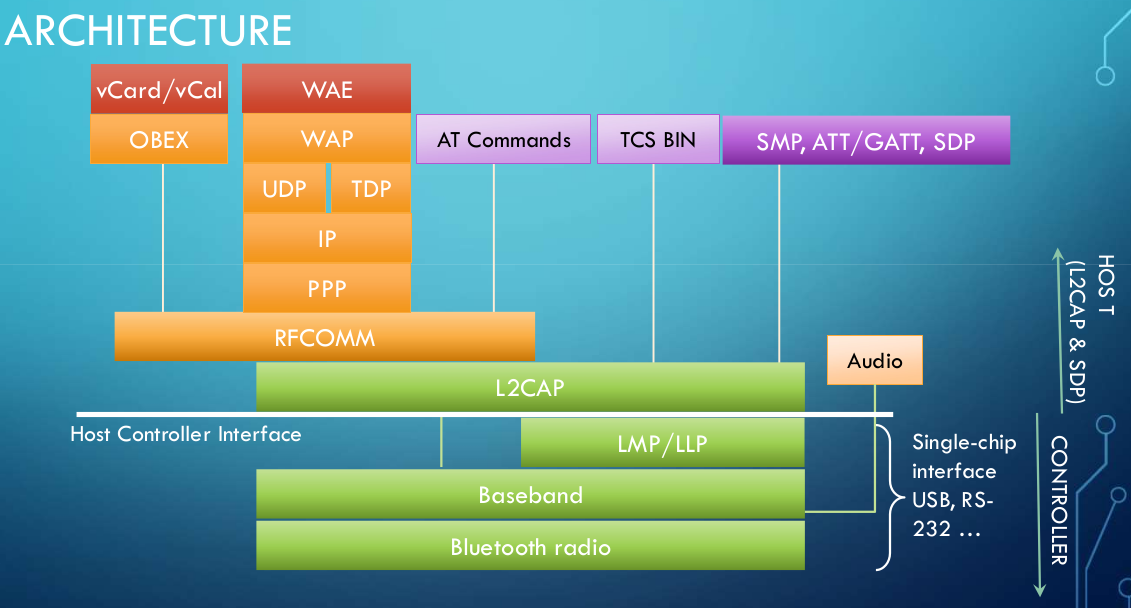
\includegraphics{images/bluetooth_architecture.png}
   \caption{Architecture of Bluetooth.}
   \label{fig:bluetooth_architecture}
\end{figure}

The bluetooth core system is composed of one or more \textbf{controllers} and a \textbf{host}. The controller is a microcontroller that executes the physical layer and the link layer, while the host is a microcontroller that executes the higher layers of the protocol stack. The host communicates with the controller through a serial interface.\\
The host comprises all layer below the HCI (Host Controller Interface) shown in Fig. \ref{fig:bluetooth_architecture} , while the controller comprises the HCI and the layers below.

\note{TODO check this}

The core protocols are various:
\begin{itemize}
   \item \textit{Radio}: defines the specification of the radio frequencies.
   \item \textit{Baseband}: defines the low level procedures of the PHY layer
   \item \textit{LMP} (link management protocol - for \texttt{BR/EDR}) / \textit{LLP} (link layer protocol - for \texttt{BLE}): setup and control of the link.
   \item \textit{HCI} (Host Controller Interface): interface between hardware and software.
   \item \textit{L2CAP} (Logical Link Control and Adaptation): higher-level protocol multiplexing,
   packet segmentation and reassembly, and the conveying of quality of service information.
   \begin{itemize}
      \item Provides an interface to higher level protocols and applications to transmit and receive data packets, up
      to 64 kilobytes in length.
      \item Implements flow control and retransmission modes.
   \end{itemize}
   \item \textit{SDP}: Service Discovery Protocol
\end{itemize}

\subsection{\texttt{BR/EDR} vs \texttt{BLE}}
BR/EDR (Basic Rate/Enhanced Data Rate), used for streaming audio and other data. It is a point-to-point connection, and can connect up to 7 devices.\\
It is connection-oriented, meaning that the a link between two devices is kept even if no data is flowing;
There are however \textit{sniff modes} which allow devices to sleep and thus to save energy.\\
Peak transmit current is about $25mA$, which is low compared to other wireless technologies, but still not enough low for very low-power devices or coin cell batteries.
\nl

BLE (Bluetooth Low Energy) is a different protocol, designed for ultra low power consumption. It is connectionless, and can connect up to 40 devices.\\
It exploits short packets to reduce TX peak current and RX time, and less channels to improve discovery and connection time, ultimately resulting in overall lower power consumption, with $20mA$ as peak transmit current, and $6\mu A$ as average current.

BLE operates at 2.4GHz and uses 40 channels with FDMA (Frequency Division Multiple Access), with 2MHz spacing. IChannels 37,38,39 are used for connection, discovery and broadcast, while the others for data.
The maximum data rate is $1Mbps$, however this protocol is meant for smaller packets, it is not optimized for file transferring.\\
Each channel is divided into time units (events), either
\begin{itemize}
   \item \textit{Advertising} events
   \item \textit{Connection} events
\end{itemize}


\section{Network topologies}
\begin{paracol}{2}
   
   Two topologies are possible, \textit{Piconet} and \textit{Scatternet}.
   The Scatternet is a network of Piconets, where a device can be part of multiple Piconets, and thus can act as a bridge between them.

   The master is unique in each piconet and synchronizes it, besides it also controls the access to the channel of all slave stations.\\
   In BE/EDR up to 7 slaves can be connected to a master, while in BLE there is no limit, but a device may be in only one piconet.
   \switchcolumn
   \begin{figure}[htbp]
      \centering
      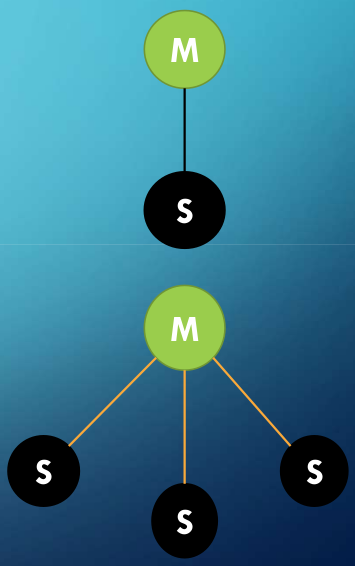
\includegraphics[width=0.45\columnwidth]{images/bluetooth_topology.png}
      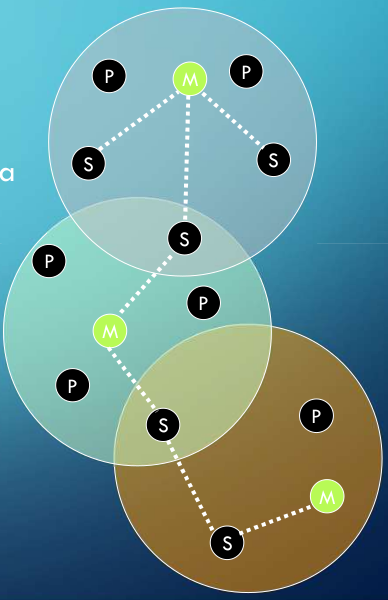
\includegraphics[width=0.45\columnwidth]{images/bluetooth_scatternet.png}
      \caption{Devices sharing the same channel form a \textit{Piconet}, with one Master and ---possibly--- multiple slaves.\\
      Multiple Piconets can be connected to form a \textit{Scatternet}.}
      \label{fig:bluetooth_topology}
   \end{figure}
\end{paracol}

\newpage
\section{Baseband layer}
\section{Phyisical Layer}
\begin{figure}[htbp]
   \centering
   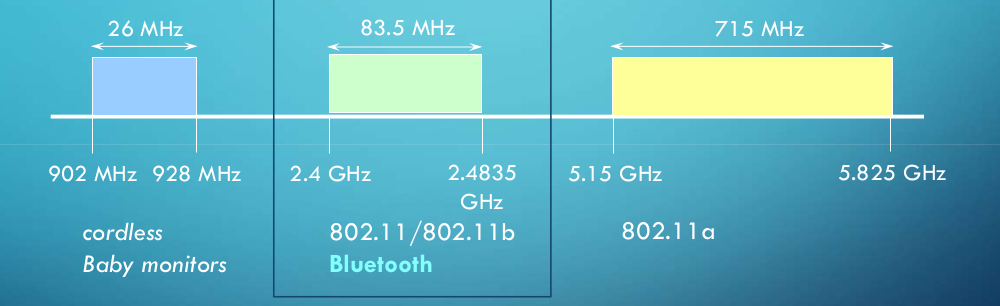
\includegraphics{images/bluetooth_frequencies.png}
   \caption{Operating bluetooth frequencies}
   \label{fig:bluetooth_frequencies}
\end{figure}

\section{Substates}
The BLE protocol defines many substates, which are used to manage the power consumption of the device. The device can switch between these states depending on the activity it is performing.

\labelitemize{Conn Establishment}{
   \begin{itemize}
      \item Page
      \item Page scan
      \item Page response
      \item Inquiry
      \item Inquiry scan
      \item Inquiry response
   \end{itemize}
}

\labelitemize{Conn state}{
   \begin{itemize}
      \item Active mode
      \item Sniff mode
      \item Hold mode
      \item Park
   \end{itemize}
}